%!TEX root = ./report.tex
\section{Solution}
\label{sec:solution}
The solution combines several open source technologies to attain an extensible solution with two reusable MWE2 client side workflows at its core. The setup allows the user to edit a subset of IFC in a generated Eclipse editor in between the two workflows. The main model is stored on a BIMServer for merging, versioning and extensibility purposes, as this section will further explain. The fact that the solution is open source means that it is not tied to any one company or organisation, unlike most BIM software.

\subsection{IFC Meta Model}
\label{subsec:ifc_meta_model}
Fundamental to the solution is in which format we work with IFC buildings. We first examined the IFC meta model used by the BIMServer project. Serializers for both the EXPRESS and XML versions of IFC exists for this meta model, although they are very tightly coupled with the rest of the BIMServer project, making them hard to use without including large parts of the BIMServer source in our solution. Further, this meta model has some undesirable features, such as references being modeled as strings, instead of pointing directly to the elements in question.

Instead, we chose to auto generate the model based on the XML Schema Definition (XSD) for ifcXML. This generated model also includes serializers for ifcXML, but not for IFC-EXPRESS. As the files are served through BIMServer, this is not a problem, since BIMServer can accept many different formats, and output ifcXML from them. This solution has the benefit that when the ifcXML schema is updated, it is trivial to produce a new meta model. A drawback is that the generated meta model has many more elements than the one from BIMServer, as it contains wrapper elements for most object types. Several other problems were encountered due to the large size of IFC. These are described in Section \ref{subsec:requirements_evaluation}.

\subsection{Pipes DSL}
\label{subsec:pipes_dsl}
Before moving into a more technical description of the workflows facilitating the end solution we here present the simple Pipes DSL, which works as the solution front end.

\begin{figure}[t]
    \centering
        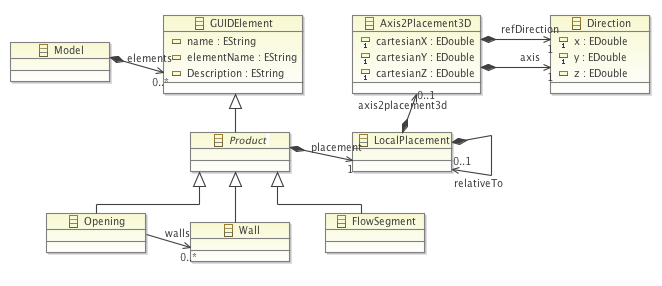
\includegraphics[width=110mm]{images/PipesEcoreModel.png}
    \caption{Pipes DSL Ecore Model}
    \label{fig:pipes_dsl_ecore_model}
\end{figure}

Figure \ref{fig:pipes_dsl_ecore_model} shows the Ecore model that the DSL is built on. Compared to Figure \ref{fig:ifcheirachy} all the critical elements of the domain are still present, but the inheritance hierarchy has been greatly simplified. As it can be seen Wall, Opening and Pipe are top level elements each with a physical location specified by the LocalPlacement reference. Figure (TODO INSERT IMAGE) depicts an example of an opening and a pipe as they are defined in an uncluttered and easily manageable way, compared to the EXPRESS format.

\subsection{BIMServer}
The overall workflow of the end product is depicted in Figure \ref{fig:overall_product_workflow}. As described in Kaj Jørgensen's workflow document\,\cite{jorgensen12} a construction model and a plumbing model are combined into one single model that needs to be verified for consistency. So called openings, i.e. holes in walls and floors need to be in place where the plumbing model describes flow segments to be installed. The merging of these models is executed on the BIMServer by the user as the first step of the workflow. When merging has finished, the client side of the solution can retrieve the merged building as XML. The user is now allowed to edit and add elements to the subset of the model on the client side before saving the building back to the BIMServer as XML.

Note that the solution does not take concurrent editing by multiple clients into account although the BIMServer does support version control as well as merging. We will leave it for future work to ensure correct handling of current editing by clients.

\begin{figure}[t]
    \centering
        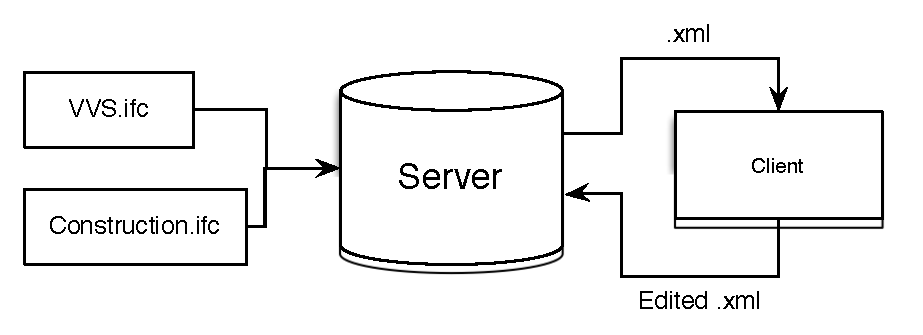
\includegraphics[width=70mm]{images/CompleteWorkflow.pdf}
    \caption{Overall product porkflow starting with merging of two models. The user can edit a subset of the model through the client-side application.}
    \label{fig:overall_product_workflow}
\end{figure}

We let a BIMServer handle the initial merging of plumbing and construction models although many tools exist for this job. The special advantage of the BIMServer is that it also provides, conversion tools allowing the user to retrieve the saved building in other formats as well as Java client library in addition to the above mentioned version control features. In particular the Java client library is important for automating the workflow, as it allows for programmatic server communication.

\subsection{Client Side}
Figure \ref{fig:IFC2PipesWorkflow} shows the IFC to Pipes workflow retrieving an IFC model from the BIMServer as XML, processing it to the corresponding Java object graph, extracting the pipes and opening elements and converting these to an editable DSL instance, which is in turn saved to disk as an XMI file. The XML file loaded from the server is saved to the local disk for use by the second workflow explained below.

\begin{figure}[t]
    \centering
        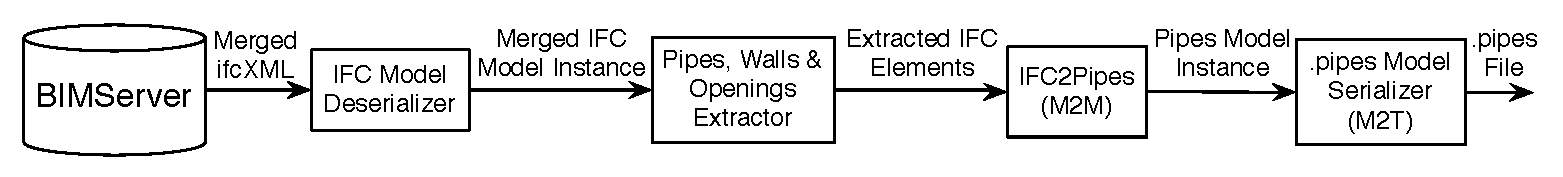
\includegraphics[width=120mm]{images/IFC2Pipes.pdf}
    \caption{Client-side workflow. Processes ifcXML from BIMServer and outputs a .pipes file, loadable in the Pipes DSL editor.}
    \label{fig:IFC2PipesWorkflow}
\end{figure}

The extraction process where relevant IFC elements are collected from the main model for conversion is implemented by a simple filtering mechanism extracting the pipe and opening elements. The real work of the IFC to Pipes workflow is done when this extract is converted to the corresponding Pipes DSL instance in the second to last step of the workflow. By utilizing the convenient model to model transformation language features of the Xtend language, each object is transformed from the IFC model to the corresponding PipesDSL object. Every IFC object inside the solution domain specified in Section \ref{subsec:problem_analysis} has a transformation rule specified here, making the conversion possible.

The second client side MWE2 workflow, Pipes to IFC, is depicted on Figure \ref{fig:Pipes2IFCWorkflow}, where the user-edited XMI file is loaded into a Main Model Updater workflow component together with the non-updated extracted instance of the main model. Notice how the extraction is loaded in using the same workflow modules as in the first workflow, except the XML file is not fetched from the server but from the local disk. This makes for an easier update process in the Main Model Updater as the extracted instance is guaranteed not to have changed while the user was editing the XMI file. After the main model instance has been updated to reflect the users changes it is converted to XML and this new file is saved back to the BIMServer.

\begin{figure}[t]
    \centering
        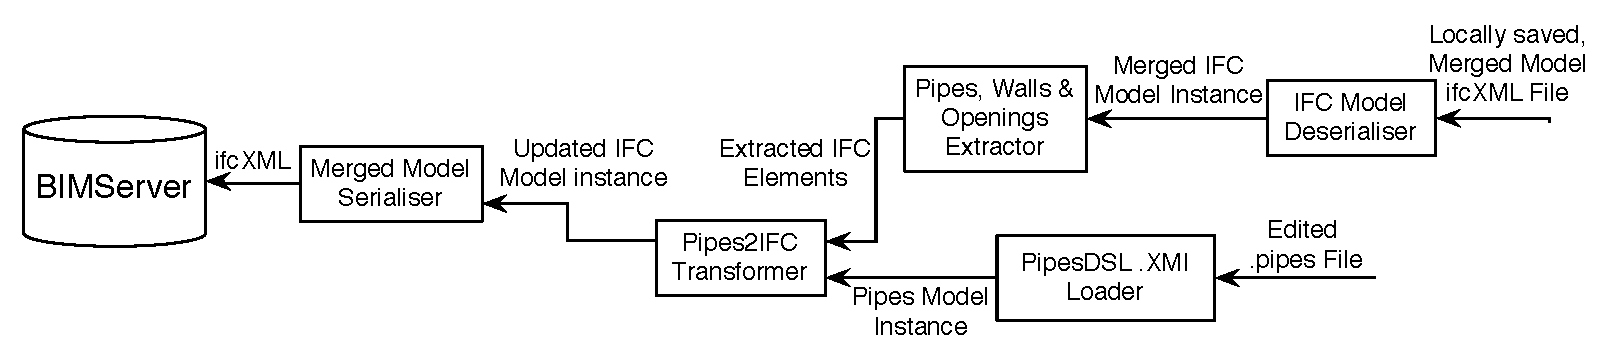
\includegraphics[width=120mm]{images/Pipes2IFC.pdf}
    \caption{Client-side workflow. First it updates the main IFC model with the changes written in the Pipes DSL editor, then sends the main model back to BIMServer.}
    \label{fig:Pipes2IFCWorkflow}
\end{figure}

Clearly, most of the work in this workflow lies with the Main Model Updater, which uses a pattern match-like dispatch language feature of Xtend to elegantly update the Java object graph of the extracted model. The routine runs through all elements in the Java object graph to update the corresponding Pipes DSL objects by looking at matching GUIDs. Only traversing an extract of the main model guarantees a better running time and still guarantees a correct update procedure, as the Pipes DSL does not allow any updates to elements outside of this extract anyway.

\paragraph{Adding and Removing} The setup not only supports updating the attributes of elements, it also allows the user to do structural changes on the model. The Main Model Updater looks for elements in the Pipes DSL object graph without a GUID to determine if a new element should be created in the IFC model. This feature allows the user to add missing openings for pipe segments and is therefore crucial for the usefulness of the end product.

Likewise, if the updater fails to find an element in Pipes DSL object graph that corresponds to the existing one in the Java object graph it means the element has been deleted and that the Main Model Updater should take appropriate action to update references
